% !TeX spellcheck = en_US
\chapter{Mean-Field Theory of a Bose Gas}%
\label{chap:mean-field-theory}


In this chapter we present the basic theory employed to study many-body quantum
systems, along with theoretical results we have obtained for ideal Bose gases
subject to periodical potentials.


\section{The weakly-interacting Bose gas}
\label{sec:the-weakly-interacting-bose-gas}

A weakly-interacting gas is a system such that the range of the inter-atomic
interactions is much smaller than the interparticle distance. For a system with
$N$ particles within a volume $V$ the distance between bosons is given in terms
of the average density $\density = N / V$ as $d = \density^{-1/3}$. The previous
assumptions have an important physical consequence, as the collisions between
two bosons can be described in terms of the asymptotic expression for its wave
function in the relative coordinate. Even more, when we only consider gases
close to zero temperature (or far below than its Bose-Einstein critical point)
we can restrict only to low values of the momenta, and from standard scattering
theory we know that the asymptotic wave function is entirely defined by lowest
order $s$-wave scattering length $\as$. So we expect that all the effects of the
interaction on the physical properties of the bosons are defined by just one
single parameter, $\as$. The diluteness condition can be written as
%\cite{bib:pitaevskii-stringari-bec.2003, bib:pethick-smith-bec-2008}
%
\begin{equation}
  \label{eq:diluteness-condition}
  |\as| \ll n^{-1/3},
\end{equation}
%
or as $n |\as|^3 \ll 1$.

We can write the Hamiltonian of the system in therms of field creation and
annihilation operators $\qmop{\Psi}^\dagger$ and $\qmop{\Psi}$,
%
\begin{equation}
  \label{eq:hamiltonian-second-quant}
  \qmop{H} = \int \frac{\hbar^2}{2m}\nabla \qmop{\Psi}^\dagger \nabla \qmop{\Psi} \; d\vec r +
  \frac{1}{2}\int \qmop{\Psi}^\dagger(\vec r) \qmop{\Psi}^\dagger(\vec r')  V(\vec r' - \vec r) \qmop{\Psi}(\vec r') \qmop{\Psi}(\vec r) \; d \vec r' d \vec r,
\end{equation}
%
where we have implicitly assumed that the field operators depend on the time,
i.e., $\qmop{\Psi}(\vec r) \equiv \qmop{\Psi}(\vec r, t)$. The annihilation and
creation operators satisfy the common commutation relations
%
\begin{align}
  \left[ \qmop{\Psi}(\vec r), \qmop{\Psi}^\dagger(\vec r') \right] = \delta(\vec r - \vec r'), \quad \left[ \qmop{\Psi}^\dagger(\vec r), \qmop{\Psi}^\dagger(\vec r') \right] =
  \left[ \qmop{\Psi}(\vec r), \qmop{\Psi}(\vec r') \right] = 0.
\end{align}
%
For a system with volume $V$ we can express the field operators as a linear
combination of creation operators of a boson with momentum $\vec p$ times a
plane wave,
%
\begin{equation}
  \qmop{\Psi}(\vec r) = \sum_{\vec p} \anhop_{\vec p} \frac{1}{\sqrt{V}} e^{i \vec p \cdot \vec r / \hbar}.
\end{equation}
%
Substituting the last expression in \eqref{eq:hamiltonian-second-quant} we
obtain the result
%
\begin{equation}
  \qmop{H} = \sum_{\vec p} \frac{p^2}{2m} \crtop_{\vec p} \anhop_{\vec p} +
  \frac{1}{2V} \sum_{\vec p_1, \vec p_2} \sum_{\vec p'} V_{\vec p'} \crtop_{\vec p_1 + \vec p'} \crtop_{\vec p_2 - \vec p'} \anhop_{\vec p_2} \anhop_{\vec p_1},
\end{equation}
%
where
%
\begin{equation}
  V_{\vec p'} = \int  d\vec r \, V(\vec r) e^{-i \vec p' \cdot \vec r / \hbar}.
\end{equation}
%
Previously we have emphasized that, in virtue of the diluteness criteria, the
physics of the system depends only on the scattering length $\as$, not in the
shape of the two-body potential. Therefore, we can replace the physical two-body
potential with an \textit{effective} soft potential $V_\mathrm{eff}$ that gives
the correct value of the scattering length. For low momenta we only have to
consider the case $\vec p' = 0$, hence the Hamiltonian can be reduced to
%
\begin{equation}
  \label{eq:gp-lowest-order-hamiltonian}
  \qmop{H} = \sum_{\vec p} \frac{p^2}{2m} \crtop_{\vec p} \anhop_{\vec p} +
  \frac{V_{\vec 0}}{2 V} \sum_{\vec p_1, \vec p_2} \sum_{\vec p'} \crtop_{\vec p_1 + \vec p'} \crtop_{\vec p_2 - \vec p'} \anhop_{\vec p_2} \anhop_{\vec p_1},
\end{equation}
%
with $V_{\vec 0} = \int d \vec r \, V_\mathrm{eff}(\vec r)$. The theory of
diluted gases requires the Bogoliubov prescription in which we replace the
creation and annihilation operators for $c$-numbers,
%
\begin{equation}
  \anhop_\vec{0} = \sqrt{N_\vec{0}},
\end{equation}
%
where $N_\vec{0}$ is the number of bosons in the ground state of the system. As
we are considering that the system is at temperatures far below the BEC critical
temperature, then it is reasonable to assume that, even when the occupation of
states with momenta $\vec p \neq \vec 0$ is small, it is negligible compared to
the occupation to the ground state. Hence practically all the $N$ bosons in the
system occupy the ground state and $N_{\vec 0} \sim N$, then $\anhop_{\vec{0}}
  \sim \sqrt{N}$ and only the ground state will contribute to the second term of
\eqref{eq:gp-lowest-order-hamiltonian}. Then the first term of the same equation
will be zero as it depends on $p^2$. The ground state energy of the system will
be
%
\begin{equation}
  E_{\vec 0} = \frac{1}{2} \frac{N^2 V_{\vec 0}}{V}.
\end{equation}
%
The constant $V_{\vec 0}$ can also be related to the scattering length using the
first approximation of the Born series \cite{bib:pethick-smith-bec-2008},
%
\begin{equation}
  V_{\vec 0} = \frac{4 \pi \hbar^2 \as}{m}.
\end{equation}
%
In terms of the density $n = N / V$ the energy of the ground state is given as
%
\begin{equation}
  \label{eq:gross-pitaevskii-ground-state-energy}
  E_{\vec 0} = \frac{1}{2} g n N,
\end{equation}
%
with the interaction parameter
%
\begin{equation}
  \label{eq:gross-pitaevskii-interaction-parameter}
  g = \frac{4 \pi \hbar^2 a }{m}.
\end{equation}
%
Therefore the chemical potential is
%
\begin{equation}
  \label{eq:gross-pitaevskii-chemical-potential}
  \mu = \frac{\partial E_{\vec 0}}{\partial N} = g n.
\end{equation}
%
The chemical potential is nonzero, in contrast to the case of a noninteracting
Bose gas. This formula naturally goes to case of the ideal gas when the
interaction, i.e., $g$, tends to zero.


\section{The Gross-Pitaevskii equation}

We can obtain the Hamiltonian of the weakly interacting Bose gas subject to an
external potential starting from the Hamiltonian in terms of the creation and
annihilation field operators
%
\begin{equation}
  \label{eq:hamiltonian-full-second-quant}
  \qmop{H} = \int {\Psi}^\dagger(\vec r) \qmop{H}_0(\vec r) \qmop{\Psi}(\vec r) \; d\vec r +
  \frac{1}{2} \int \qmop{\Psi}^\dagger(\vec r) \qmop{\Psi}^\dagger(\vec r')  V(\vec r' - \vec r) \qmop{\Psi}(\vec r') \qmop{\Psi}(\vec r) \; d \vec r' d \vec r.
\end{equation}
%
The operator $\qmop{H}_0(\vec r)$ is the Hamiltonian of the non-interacting
Bose gas subject to the external potential
%, namely $\qmop{V}_\mathrm{ext}(\vec r)$,
%
\begin{equation}
  \label{eq:non-interacting-hamiltonian}
  \qmop{H}_0(\vec r) = \frac{\qmop{p}^2}{2m} + \qmop{V}_\mathrm{ext}(\vec r).
\end{equation}
%
If we again consider a weakly interacting Bose gas then we know from the
previous discussion that the interaction between the bosons is determined
entirely by the $s$-wave scattering length $\as$, so the shape of the
interaction potential does not matter as long as it yields the correct value of
the scattering length. It's a common practice to replace the interaction
potential by a contact pseudo-potential
%
\begin{equation}
  V(\vec r - \vec r') = g \delta(\vec r - \vec r').
\end{equation}
%
where $g = 4 \pi \hbar^2 a / m$. This leads us to the Hamiltonian
%
\begin{equation}
  \label{eq:pseudo-potential-hamiltonian}
  \qmop{H} = \int \left({\Psi}^\dagger(\vec r) \qmop{H}_0(\vec r) \qmop{\Psi}(\vec r) +
  \frac{g}{2} \qmop{\Psi}^\dagger(\vec r) \qmop{\Psi}^\dagger(\vec r) \qmop{\Psi}(\vec r) \qmop{\Psi}(\vec r)\right)  d \vec r.
\end{equation}

To find the wave function of the system implies to find the field operator
$\qmop{\Psi}(\vec r, t)$. We could in principle find the field operator as a
function of the time from the Heisenberg equation,
%
\begin{equation}
  \label{eq:heisenberg-equation}
  i \hbar \frac{\partial \qmop{\Psi}(\vec r, t)}{\partial t} = -\left[\qmop{H}(t), \qmop{\Psi}(\vec r, t)\right].
\end{equation}
%
The expression for the Hamiltonian is given by Eq.
\eqref{eq:pseudo-potential-hamiltonian}, where we have implicitly stated that
$\qmop{H} \equiv \qmop{H}(t)$ is a function of the time as the field operators
$\qmop{\Psi}(\vec r, t)$ depend on the time as well. Equation
\eqref{eq:heisenberg-equation} yields the corresponding equation
%
\begin{equation}
  \label{eq:gross-pitaevskii-heisenberg-equation}
  i\hbar \frac{\partial \qmop{\Psi}(\vec r, t)}{\partial t} = \qmop{H}_0 \qmop{\Psi}(\vec r, t) +
  g \, \qmop{\Psi}^\dagger(\vec r, t) \qmop{\Psi}(\vec r, t) \qmop{\Psi}(\vec r, t).
\end{equation}
%
As in the case of an interacting homogeneous Bose gas, we regard the field
operator $\qmop{\Psi}(\vec r, t)$ as a classical field ---a $c$-field---
$\Phi(\vec r, t)$ assuming that practically all the bosons occupy the ground
state of the system and neglecting quantum fluctuations. The $c$-field
$\Phi(\vec r, t)$ represents the  wave function of the condensed bosons as a
whole, is also called the order parameter of the condensate. The equation for
$\Phi(\vec r, t)$ then becomes
%
\begin{equation}
  \label{eq:gross-pitaevskii-equation-3d}
  i\hbar \frac{\partial \Phi}{\partial t} = -\frac{\hbar^2}{2m} \nabla^2 \Phi(\vec r, t) +
  V_\mathrm{ext}(\vec r) \Phi(\vec r, t) +
  g \left| \Phi(\vec r, t) \right|^2 \Phi(\vec r, t),
\end{equation}
%
which is the celebrated \textit{Gross-Pitaevskii equation}
\cite{bib:gross-il-nuovo-cimento.1961, bib:pitaevskii-jetp.1961} in three
dimensions and is used to model a weakly-interacting inhomogeneous Bose gas.
This equation is identical to the one-body Schrödinger equation for a single
particle, with the important difference that it includes a nonlinear term that
accounts for the interactions between the bosons and that is proportional to the
square of the wave function of the condensate.

The Gross-Pitaevskii equation is valid to describe phenomena that occurs for
weakly interacting systems at scales that are far larger than the scattering
length and at temperatures low enough. The assumption that the vast majority of
the bosons occupy the ground state allow us to assert that the density of the
condensate is the density of the gas,
%
\begin{equation}
  \textit{}   n(\vec r) = \left| \Phi(\vec r) \right|^2,
\end{equation}
%
and that the total number of bosons $N$ is
%
\begin{equation}
  N = \int n(\vec r) \, d\vec r.
\end{equation}
%
This equation known as the normalization condition, fixes the chemical potential
$\mu$ of the condensate.

Equation \eqref{eq:gross-pitaevskii-equation-3d} has a particular family of
stationary solutions of the form
%
\begin{equation}
  \Psi(\vec r, t) = \Psi(\vec r) e^{-i\mu t /\hbar}
\end{equation}
%
where the chemical potential fixes the time dependence of the wave function. The
Gross-Pitaevskii equation takes the simpler form
%
\begin{equation}
  \label{eq:gross-pitaevskii-equation-3d-stat}
  -\frac{\hbar^2}{2m} \nabla^2 \Phi(\vec r) +
  V_\mathrm{ext}(\vec r) \Phi(\vec r) +
  g \left| \Phi(\vec r) \right|^2 \Phi(\vec r) = \mu \Phi(\vec r),
\end{equation}
%
commonly known as the stationary \textit{Gross-Pitaevskii equation}.

The energy of the condensate will become a functional of the solutions of
\eqref{eq:gross-pitaevskii-equation-3d-stat} and is expressed as
%
\begin{equation}
  \label{eq:gross-pitaevskii-energy}
  E[\Phi] = \int d\vec r \, \left[
    \frac{\hbar^2}{2m} |\nabla \Phi|^2 + V_\mathrm{ext}(\vec r) |\Phi|^2 +
    \frac{g}{2} |\Phi|^4
    \right],
\end{equation}
%
along with the relation
%
\begin{equation}
  \label{eq:gross-pitaevskii-energy-chemical-potential}
  \mu = \frac{\partial E}{\partial N}.
\end{equation}



\section{Mean-field theory in one dimension}
\label{sec:mean-field-theory-in-one-dimension}

The theory of diluted gases described in the previous section has been done for
a three-dimensional system. However, with today's experimental techniques it is
possible to confine a Bose fluid within highly anisotropic potentials that
effectively constrain the movement of the particles in one, two or even in three
spatial dimensions \cite{bib:a-gorlitz-phys-rev-lett.87.130402,
  bib:paredes-bloch-et-al-nature.419.2014}. If we want to apply the previous
theory it is necessary to adjust it in order to know under which conditions the
mean-field picture is valid.

Let's point out that one criteria to discard or assert the applicability of
mean-field theory for a homogeneous Bose gas requires that the average distance
between bosons be smaller than the healing length of the gas
%
\begin{equation}
  \label{eq:healing-length}
  \xi = \frac{1}{\sqrt{8 \pi n \as}},
\end{equation}
%
with $\as$ the $s$-wave scattering length and $n = N/V$ the average
(three-dimensional) particle density. In the case of a trapped gas the previous
expression give us an estimate of the order of magnitude of the healing length
because the density is not uniform. The healing length is also related to the
sound velocity $c$ in the fluid as
%
\begin{equation}
  \label{eq:healing-length-sound-velocity}
  \xi = \frac{\hbar}{\sqrt{2} m c}.
\end{equation}
The average distance $d$ between particles can also be given in terms of the
density $n$ in a roughly way as $d = n^{-1/3}$, hence the ratio $\xi / d$ is
proportional to $(na^3)^{-1/6}$. This implies that the condition $\xi > d$ is
well satisfied for small densities, supporting the fact that the
Gross-Pitaevskii equation is suited only for diluted gases. However, if we
change the geometry of the system and reduce the dimensionality the situation
may be completely different.

Let's consider the case of a gas confined in a cylindrical geometry of length
$L$ produced by an harmonic potential $V(r_{\bot}) = (m/2)\omega^2_{\bot}
  r^2_\bot$. When the radial trapping is  large the average linear density $n_1$
is related to the three-dimensional one through
%
\begin{equation}
  n_1 = n \pi \as^2_\bot
\end{equation}
%
where $\as_\bot = \sqrt{\hbar / m \omega_\bot}$ is the radial oscillation
length. In this geometry the density $n$ is measured at $r_\bot = 0$. In this
\emph{one-dimensional regime} the distance between particles is no longer
$n^{-1/3}$, but $d = n_1^{-1}$, so the quotient $\xi / d$ is
%
\begin{equation}
  \label{eq:mean-field-one-dim-quotient}
  \frac{\xi}{d} = \sqrt{\frac{\as^2_\bot}{8\as} n_1}.
\end{equation}
%
The meaning of this equation is that the quotient of interest becomes smaller as
the linear density decreases, just the opposite than the three-dimensional case.
The direct consequence of this is that the mean-field picture developed in the
previous section becomes inadequate for diluted systems with a one-dimensional
(or for systems with a very elongated, cigar-like) geometry!
%
Nevertheless, there is the possibility that the healing length $\xi$ be larger
than the average interparticle distance $d$ if
%
\begin{equation}
  n_1 \frac{\as^2_{\bot}}{\as} \gg 1,
\end{equation}
%
for instance, when the linear density is large enough. So the mean-field regime
for a one-dimensional system corresponds to the limit of high densities! This is
not the only possibility, as we have another relevant parameter, commonly
identified as the effective \textit{one-dimensional scattering length}
$\as_{\mathrm{1D}}$,
%
\begin{equation}
  \label{eq:one-dim-scattering-length}
  \as_{\mathrm{1D}} = \frac{\as^2_{\bot}}{\as}.
\end{equation}
%
The mean-filed theory picture will be valid when $\as_{\bot} \gg \as$ also. The
relevant condition that must be fulfilled in order to apply mean-field theory in
one-dimension is commonly stated as
%
\begin{equation}
  n_1 \as_\mathrm{1D} \gg 1.
\end{equation}
%
The factor $n_1 \as_\mathrm{1D}$ is known as the \emph{gas parameter}, and the
relevant physical properties of the system as the energy, the static structure
factor and the momentum distribution may be stated in terms of it.

Going back to the case of a homogeneous gas with a cylindrical geometry
generated by an axial harmonic potential, we can recognize two-regimes
\cite[pp~325]{bib:pitaevskii-stringari-bec.2003}:

\begin{itemize}
  \item $n_1 \as \gg 1$, known as the Thomas-Fermi regime or three-dimensional
        cigar. In this regime we have many excited configurations of the
        harmonic oscillator in the radial direction. By neglecting the
        kinetic-energy in the radial direction and the normalization condition
        we can find the chemical potential as
        %
        \begin{equation}
          \frac{\mu}{\hbar \omega_\bot} = 2(a n_1)^{1/2}
        \end{equation}
        The system locally resembles a three-dimension system, but geometrically
        looks one-dimensional.

  \item $n_1 \as \ll 1$, known as the one-dimensional mean field regime. Only
        the ground state of the harmonic oscillator in the radial direction
        contributes to the energy. The chemical potential of the gas is
        %
        \begin{equation}
          \label{eq:gross-pitaevskii-cigar-like-chemical-potential}
          \frac{\mu}{\hbar \omega_\bot} = 1 + 2 a n_1.
        \end{equation}
        %
        The constant term arises from the zero-point motion energy of the ground
        state, while the second term is identified as the chemical potential of
        the one-dimensional mean field regime. i.e,
        %
        \begin{equation}
          \frac{\mu_\mathrm{1D}}{\hbar \omega_\bot} = 2 a n_1.
        \end{equation}
\end{itemize}
%
Our main interest is the mean-field regime, $\as n_1 \ll 1$. Considering the
definition of the effective one-dimensional scattering length, Eq.
\eqref{eq:one-dim-scattering-length}, the linear density $n_1 = N / L$ and the
harmonic radius $\as_\bot = \sqrt{\hbar / m \omega_\bot}$ we find from the
previous relation that the one-dimensional chemical potential is
%
\begin{equation}
  \mu_\mathrm{1D} = \frac{2 \hbar^2}{m \asonedim} n_1.
\end{equation}
%
With the concrete dependence of the chemical potential on the number of bosons
$N$ and Eq. \eqref{eq:gross-pitaevskii-energy-chemical-potential} we obtain the
energy of the Bose gas:
%
\begin{equation}
  E = \frac{\hbar^2}{m \asonedim} n_1 N.
\end{equation}
%
Observing carefully these expressions and comparing them to those for the
chemical potential and the energy per boson for a three-dimensional mean field
regime, equations \eqref{eq:gross-pitaevskii-ground-state-energy} and
\eqref{eq:gross-pitaevskii-chemical-potential} respectively, we observe that
they are essentially identical if we define an equivalent interaction parameter
for one-dimensional systems, $\gonedim$, as
%
\begin{equation}
  \label{eq:gross-pitaevskii-interaction-parameter-1d}
  \gonedim = \frac{2 \hbar^2}{m \asonedim}.
\end{equation}
%
Hence we have that
%
\begin{equation}
  \label{eq:gross-pitaevskii-1d-energy}
  E = \frac{1}{2} \gonedim n_1 N
\end{equation}
%
and
%
\begin{equation}
  \label{eq:gross-pitaevskii-1d-chemical-potential}
  \mu_\mathrm{1D} = \gonedim n_1.
\end{equation}
%
%This parameter has been identified by \cite[Olshanni 1998]{bib:olshanii-phys-rev-lett.81.938} in the study of atomic
%scattering in a gas of impenetrable bosons.

Dimensional reduction methods \cite{bib:lieb-j-commun-math-Phys.224.17.2001,
  bib:cai-rosenkranzs-phys-rev-A.82.043623} applied over the three-dimensional
Gross-Pitaevskii lead us to the one-dimensional version of the same equation,
which retains the same mathematical form,
%
\begin{equation}
  \label{eq:gross-pitaevskii-equation-1d}
  -\frac{\hbar^2}{2m}\frac{d^2\Phi}{dz^2} + V_{\mathrm{ext}}(z) \Phi(z) + \gonedim |\Phi(z)|^2 \Phi(z)
  = \mu \Phi(z),
\end{equation}
%
where the interaction parameter must be changed with the adequate
one-dimensional version. The energy functional also retains an equivalent form,
%
\begin{equation}
  \label{eq:gross-pitaevskii-1d-energy-functional}
  E[\gpwavefunc] = \int dz \left( \frac{\hbar^2}{2m} \left| \frac{d\gpwavefunc}{dz} \right|^2 + V_{\mathrm{ext}}(z) \left| \gpwavefunc(z) \right|^2 + \frac{\gonedim}{2} \left| \gpwavefunc(z) \right|^4  \right).
\end{equation}


The study of the properties of a many-body, interacting quantum gas is a
challenging work. In order to analyze the properties of these systems several
approaches can be taken. One of them, which we explain in this section of our
work, addresses the problem of a dilute, interacting Bose gas in 1D at zero
temperature using the stationary Gross-Pitaevskii equation,
%
\begin{equation}
  -\frac{\hbar^2}{2m}\frac{d^2\Phi}{dz^2} + V_{\mathrm{ext}}(z) \Phi(z) + \gonedim |\Phi(z)|^2 \Phi(z)
  = \mu \Phi(z),
\end{equation}
%
where $\Phi(z)$ represents the wave function of the ground state of the gas,
$\mu$ is the chemical potential of the system and $\gonedim$ is the interaction
strength factor, $\gonedim = {2\hbar^2}/{m \asonedim}$. The effective
one-dimensional scattering length $\asonedim$ can only be positive for a free
gas --a repulsive interaction-- because of the requirement of thermodynamic
stability %\cite[pp.~29]{bib:pitaevskii-stringari-bec.2003} but in the presence
of an  external confinement it may have any value: positive for a repulsive
interaction ($\asonedim > 0$) or negative for an attractive one ($\asonedim <
  0$). We recall that the condition that should be fulfilled in order to be
authorized to use the Gross-Pitaevskii equation in one dimension is
%
\begin{equation}
  \label{eq:mean-field-regime-condition}
  \densityone \asonedim \gg 1.
\end{equation}
%
The energy functional for the inhomogeneous 1D system is given by the equation
\eqref{eq:gross-pitaevskii-1d-energy-functional}, which reduces to $E = \gonedim
  \densityone N / 2$ for the energy of the free 1D Bose gas.


%\section{The dilute free Bose gas}
%
%The Gross-Pitaevskii equation can be applied to a dilute, interacting Bose gas subject to no external potential. In such cases



\section{Preliminary results}

\subsection{Solution of the {\GP} equation for a constant potential}

The solution of the {\GP} equation can be obtained analytically if the external
potential acting over the gas is a constant
\cite{bib:zakharov-sov-phys-jetp.34.1972, bib:smerzi-phys-rev-E.70.016605.2004,
  bib:seaman-phys-rev-A.71.033622.2005}. First of all, let's write the wave
function of the gas $\gpwavefunc(z)$ which, in general, is a complex quantity,
as
%
\begin{equation}
  \label{eq:gross-pitaevskii-wave-function}
  \gpwavefunc(z) = \sqrt{\gprho(z)} e^{i \theta(z)},
\end{equation}
%
where the real function $\gprho(z)$ turns out to be the density profile of the
gas as $\gprho(z) = |\gpwavefunc(z)|^2$, and the real function $\theta(z)$ is
the argument of the complex part of $\gpwavefunc$. Let be $u(z) =
  \sqrt{\gprho(z)}$, then the real and the complex parts of eq.
\eqref{eq:gross-pitaevskii-equation-1d} are
%
\begin{align}
  \label{eq:gross-pitaevskii-equation-real-part} -\frac{d^2 u}{dz^2} + u(z) \left(\frac{d\theta}{dz}\right)^2 + \frac{2m (V(z) - \mu)}{\hbar^2} u(z) + \frac{2 m \gonedim}{\hbar^2} u^3(z) & = 0  \\
  \label{eq:gross-pitaevskii-equation-imag-part} u(z) \frac{d^2 \theta}{dz^2}  + 2\frac{du}{dz} \frac{d \theta}{dz}                                                                        & = 0,
\end{align}
%
respectively.

The solution to equation \eqref{eq:gross-pitaevskii-equation-imag-part} can be
obtained by separation of variables as
%
\begin{equation}
  \label{eq:gross-pitaevskii-theta}
  \theta(z) = \alpha \int_{0}^{z} \frac{dz'}{u^2(z')} + \theta(z=0),
\end{equation}
%
where $\alpha$ is a constant of integration whose value is fixed by the boundary
conditions of the problem. In spite of its simplicity, equation
\eqref{eq:gross-pitaevskii-theta} is coupled with
\eqref{eq:gross-pitaevskii-equation-real-part}, as it depends on $u^2(z)$.

At this point we can not proceed any further in the quest of a solution of eq.
\eqref{eq:gross-pitaevskii-equation-real-part} as long as we do not have an
explicit expression of $V(z)$. In the case of a constant external potential
$V(z) = V_0$ we multiply \eqref{eq:gross-pitaevskii-equation-real-part} by $du /
  dz$ and then integrate so we arrive to the equation
%
\begin{equation}
  -\frac{1}{2} \left( \frac{du}{dz} \right)^2 - \frac{\alpha^2}{2 u^2} +
  \frac{1}{2} \frac{2m (V_0 - \mu)}{\hbar^2} u^2 + \frac{m \gonedim}{2 \hbar^2} u^4 = C,
\end{equation}
%
with $C$ being a constant of integration. Finally, we multiply by $-2u^2(z)$ and
rearrange terms, arriving to the differential equation
%
\begin{equation}
  \label{eq:gross-pitaevskii-equation-real-part-2}
  \frac{d u^2}{dz} = 2 \left[ \frac{m \gonedim}{\hbar^2} u^6 + \frac{2m}{\hbar^2} (V_0 - \mu) u^4 - 2 C u^2 - \alpha^2  \right]^{1/2}.
\end{equation}
%
Now we can express \eqref{eq:gross-pitaevskii-equation-real-part-2} as a
differential equation for the density, $\gprho = u^2$, as
%
\begin{align}
  \label{eq:gross-pitaevskii-density-equation}
  \left( \frac{d\gprho}{dz} \right)^2 = \frac{4 m \gonedim}{\hbar^2} \gprho^3 + \frac{8 m}{\hbar^2} (V_0 - \mu) \gprho^2 - \gpgamma \rho - 4\alpha^2,
\end{align}
%
where $\gpgamma$ equals $8C$, but we do not want to carry with the eight factor
all the time as it is not necessary. Finally the $\theta(z)$ function in terms
of the density becomes
%
\begin{equation}
  \label{eq:gross-pitaevskii-phase-equation}
  \theta(z) = \alpha \int_{0}^{z} \frac{dz'}{\gprho(z')} + \theta(z=0).
\end{equation}
%
Equations \eqref{eq:gross-pitaevskii-density-equation} and
\eqref{eq:gross-pitaevskii-phase-equation} give the full form of the ground
state wave function of the system. We have to apply the adequate boundary
conditions in order to obtain the energy of the system and the chemical
potential, among other properties.

Despite the nonlinear nature of equation
\eqref{eq:gross-pitaevskii-density-equation}, it has an analytical solution
given in terms of the \textbf{Jacobi Elliptic functions}
\cite{bib:abramowitz-stegun-1965}. The expression for the density is
%
\begin{equation}
  \label{eq:gross-pitaevskii-density}
  \gprho(z) = \gprho[0] + 4 \ellipm \lambda^2 \, \jacobisn^2 \left( \sqrt{\frac{4 m_{\mathrm{e}} \gonedim}{\hbar^2}} \lambda (z - z_0), m_{\mathrm{e}}\right),
\end{equation}
%
where $\jacobisn(u, m_{\mathrm{e}})$ is the Jacobi elliptic sine function of
argument $u$ and elliptic modulus $m_{\mathrm{e}}$, and $\gprho[0]$, $\lambda$
and $z_0$ are constants than depend on the boundary conditions of the system.
The constants $\alpha$, $\gpgamma$, as the chemical potential $\mu$ can be
expressed as
%
\begin{align}
  \mu      & = V_0 + \frac{3 \gonedim}{2} \gprho[0] + 2 \gonedim (1 + \ellipm) \lambda^2                            \\
  \alpha^2 & = \frac{m \gonedim}{\hbar^2} \gprho[0] (\gprho[0] + 4 \lambda^2) (\gprho[0] + 4 \ellipm \lambda^2)     \\
  \gpgamma & = -\frac{4mg}{\hbar^2} (3 \gprho[0]^2 + 8 \gprho[0] (1 + \ellipm) \lambda^2 + 16 \ellipm[] \lambda^4).
\end{align}



\subsection{Density in a multi-rods external potential}

When the applied external potential has a piecewise, constant magnitude, the
density of the system and the phase $\theta(z)$ are still given by
\eqref{eq:gross-pitaevskii-density} and \eqref{eq:gross-pitaevskii-theta}, but
in addition the wave function will be a piecewise function too, as the potential
itself. For a multi-rods structure modeled through a Kronig-Penney potential
with barriers of width $b$ separated one from each other by a distance $a$, the
wave function and the potential will be
%
\begin{align}
  \label{eq:gross-pitaevskii-kronig-penney-wavefunction}
  \gpwavefunc(z) = \begin{cases}
    \gpwavefunc_1(z), & V(z) = 0, \quad 0 < z < a       \\
    \gpwavefunc_2(z), & V(z) = V_0, \quad a < z < a + b
  \end{cases}.
\end{align}
%
This implies that density and the phase will be piecewise functions too, given
as
%
\begin{align}
  \label{eq:gross-pitaevskii-kronig-penney-density}
  \gprho(z) = \begin{cases}
    \gprho[10] + 4 m_{\mathrm{e}1} \lambda^2_{1} \, \jacobisn^2 \left( \sqrt{\frac{4 m_{\mathrm{e}1} \gonedim}{\hbar^2}} \lambda_{1} (z - z_{10}), m_{\mathrm{e}1}\right), & V(z) = 0   \\
    \gprho[20] + 4 m_{\mathrm{e}2} \lambda^2_{2} \, \jacobisn^2 \left( \sqrt{\frac{4 m_{e2} \gonedim}{\hbar^2}} \lambda_2 (z - z_{20}), m_{\mathrm{e}2}\right),            & V(z) = V_0
  \end{cases},
\end{align}
%
and
%
\begin{align}
  \label{eq:gross-pitaevskii-kronig-penney-theta}
  \theta(z) = \begin{cases}
    \displaystyle \alpha_{1} \int_{0}^{z} \frac{dz'}{\gprho[1](z')} + \theta_1(z=0), & V(z) = 0   \\
    \displaystyle \alpha_{2} \int_{0}^{z} \frac{dz'}{\gprho[2](z')} + \theta_2(z=0), & V(z) = V_0
  \end{cases}
\end{align}
%
respectively. The only difference between each piece of these functions is the
set of constants $\gprho[0]$, $\lambda$, $m_{\mathrm{e}}$ and $z_0$ whose values
depend on the boundary conditions of the system.

For a multi-rods system created with a Kronig-Penney potential, we impose
physically acceptable boundary conditions over the wave function
$\gpwavefunc(z)$, namely the continuity of the wave function at the interface of
the potential, i.e. $z = 0$. This means that the density $\gprho(z)$ must be
continuous at the interface in $z=0$, i.e.
%
\begin{equation}
  \label{eq:gross-pitaevskii-density-continuity}
  \gprho[1](0) = \gprho[2](0).
\end{equation}
%
In addition we impose the continuity of the wave function derivative at $z = 0$.
This implies that
%
\begin{align}
  \label{eq:gross-pitaevskii-density-derivative-continuity}
  \left. \frac{d\gprho[1]}{dz}\right|_{z=0} = \left. \frac{d\gprho[2]}{dz}\right|_{z=0} \quad \mathrm{and} \quad \alpha_1 = \alpha_2.
\end{align}
%
Given that the {\GP} equation is translation invariant under an integer multiple
of the potential period then the wave function is a Bloch wave of the form
%
\begin{equation}
  \label{eq:gross-pitaevskii-bloch-wave}
  \gpwavefunc(z) = e^{i q z} f_q(z),
\end{equation}
%
where $q$ is the momentum of the gas and $f_q(z)$ is a periodic function with
the same period than the potential, $f_q(z) = f_q(z + l)$. Comparing equations
\eqref{eq:gross-pitaevskii-wave-function} and
\eqref{eq:gross-pitaevskii-bloch-wave} we find that
%
\begin{equation}
  f_q(z) = e^{i (\theta(z) - q z)} \sqrt{\gprho(z)},
\end{equation}
%
hence, if $f_q(z)$ has the same period of the potential $l = a + b$ then the
density is also periodic, i.e., $\gprho(z) = \gprho(z + l)$. If we look at the
interfaces of the potential this condition readily becomes
%
\begin{equation}
  \label{eq:gross-pitaevskii-density-periodicity}
  \gprho[1](z = a) = \gprho[2](z = -b).
\end{equation}
%
Also we impose the condition of periodicity of the derivative,
%
\begin{equation}
  \label{eq:gross-pitaevskii-density-derivative-periodicity}
  \left. \frac{d\gprho[1]}{dz}\right|_{z=a} = \left. \frac{d\gprho[2]}{dz}\right|_{z=-b}.
\end{equation}
%
The periodicity of $f_q(z)$ also fixes the momentum of the system,
%
\begin{equation}
  \label{eq:gross-pitaevskii-system-momentum}
  q = \frac{1}{a + b} \int_{0}^{a+b} \frac{\alpha(z')}{\rho(z')} dz'.
\end{equation}
%
In addition we impose chemical equilibrium
%
\begin{equation}
  \label{eq:gross-pitaevskii-chemical-equlibrium}
  \mu_1 = \mu_2
\end{equation}
%
and the normalization of the squared value of $\gpwavefunc(z)$,
%
\begin{equation}
  \label{eq:gross-pitaevskii-normalization-condition}
  \qquad \int_{0}^{a+b} \gprho(z') \, dz' = N,
\end{equation}
%
where $N$ is the number of bosons contained within a length equal to the
potential period.


\subsection{Energy}

The total energy of a dilute Bose gas is given by eq.
\eqref{eq:gross-pitaevskii-energy}. For our multi-rods system is given by the
expression
%
\begin{align}
  \label{eq:gross-pitaevskii-energy-multirods-prev}
  \nonumber E & = \frac{\hbar^2}{2m} \int_{0}^{a+b} \frac{1}{4 \gprho(z)} \left[
    \left(\frac{d \gprho }{dz}\right)^2 + 4 \alpha^2(z)
    \right] \; dz +
  \int_{0}^{a+b} V_{\mathrm{ext}}(z) \gprho(z) \; dz +                           \\
              & \frac{\gonedim}{2} \int_{0}^{a+b} \gprho(z)^2 \; dz,
\end{align}
%
where the integrals are carried over a single period in accordance with the
normalization condition \eqref{eq:gross-pitaevskii-normalization-condition}.
From eq. \eqref{eq:gross-pitaevskii-density-equation} we note that
%
\begin{equation}
  \frac{\hbar^2}{2m} \frac{1}{4 \gprho(z)} \left[\left(\frac{d \gprho}{dz}\right)^2 + 4 \alpha^2 \right] =
  \frac{\gonedim}{2} \gprho^2(z) + (V_{\mathrm{ext}}(z)  - \mu) \gprho(z) - \frac{\hbar^2}{8 m} \gpgamma,
\end{equation}
%
so we rewrite the first integral in the equation
\eqref{eq:gross-pitaevskii-energy-multirods-prev} as
%
\begin{align}
  \label{eq:gross-pitaevskii-energy-multirods}
  \nonumber E = \int_{0}^{a+b} (V_{\mathrm{ext}}(z) - \mu) \gprho(z) & \; dz -
  \frac{\hbar^2}{8m} \int_{0}^{a+b} \gpgamma(z) \; dz +                                                                     \\
                                                                     & \int_{0}^{a+b} V_{\mathrm{ext}}(z) \gprho(z) \; dz +
  \gonedim \int_{0}^{a+b} \gprho^2(z) \; dz.
\end{align}
%
In this equation we have expressed the external potential and the constant
$\gpgamma$ as functions of $z$, but we must always take into account that they
are constants that have different values depending on which interval $z$ is
located. The definition of $V_{\mathrm{ext}}(z)$ is given in
\eqref{eq:gross-pitaevskii-kronig-penney-wavefunction}.


\subsection{Numerical results}

We are particularly interested in the solutions of the Gross-Pitaevskii equation
for the lowest momentum, $q = 0$, as we can compare the energy for this case
with the energy obtained through Variational Monte Carlo method and with the
exact results obtained from the Lieb-Liniger theory. This also fixes the
parameter $\alpha$ to zero so the current
%
\begin{equation}
  j(z) = \gprho(z) \frac{\hbar}{m} \frac{d\theta}{dz} = \frac{\hbar}{m} \alpha
\end{equation}
%
is zero as well.
%
\begin{figure}[t!]
  \centering
  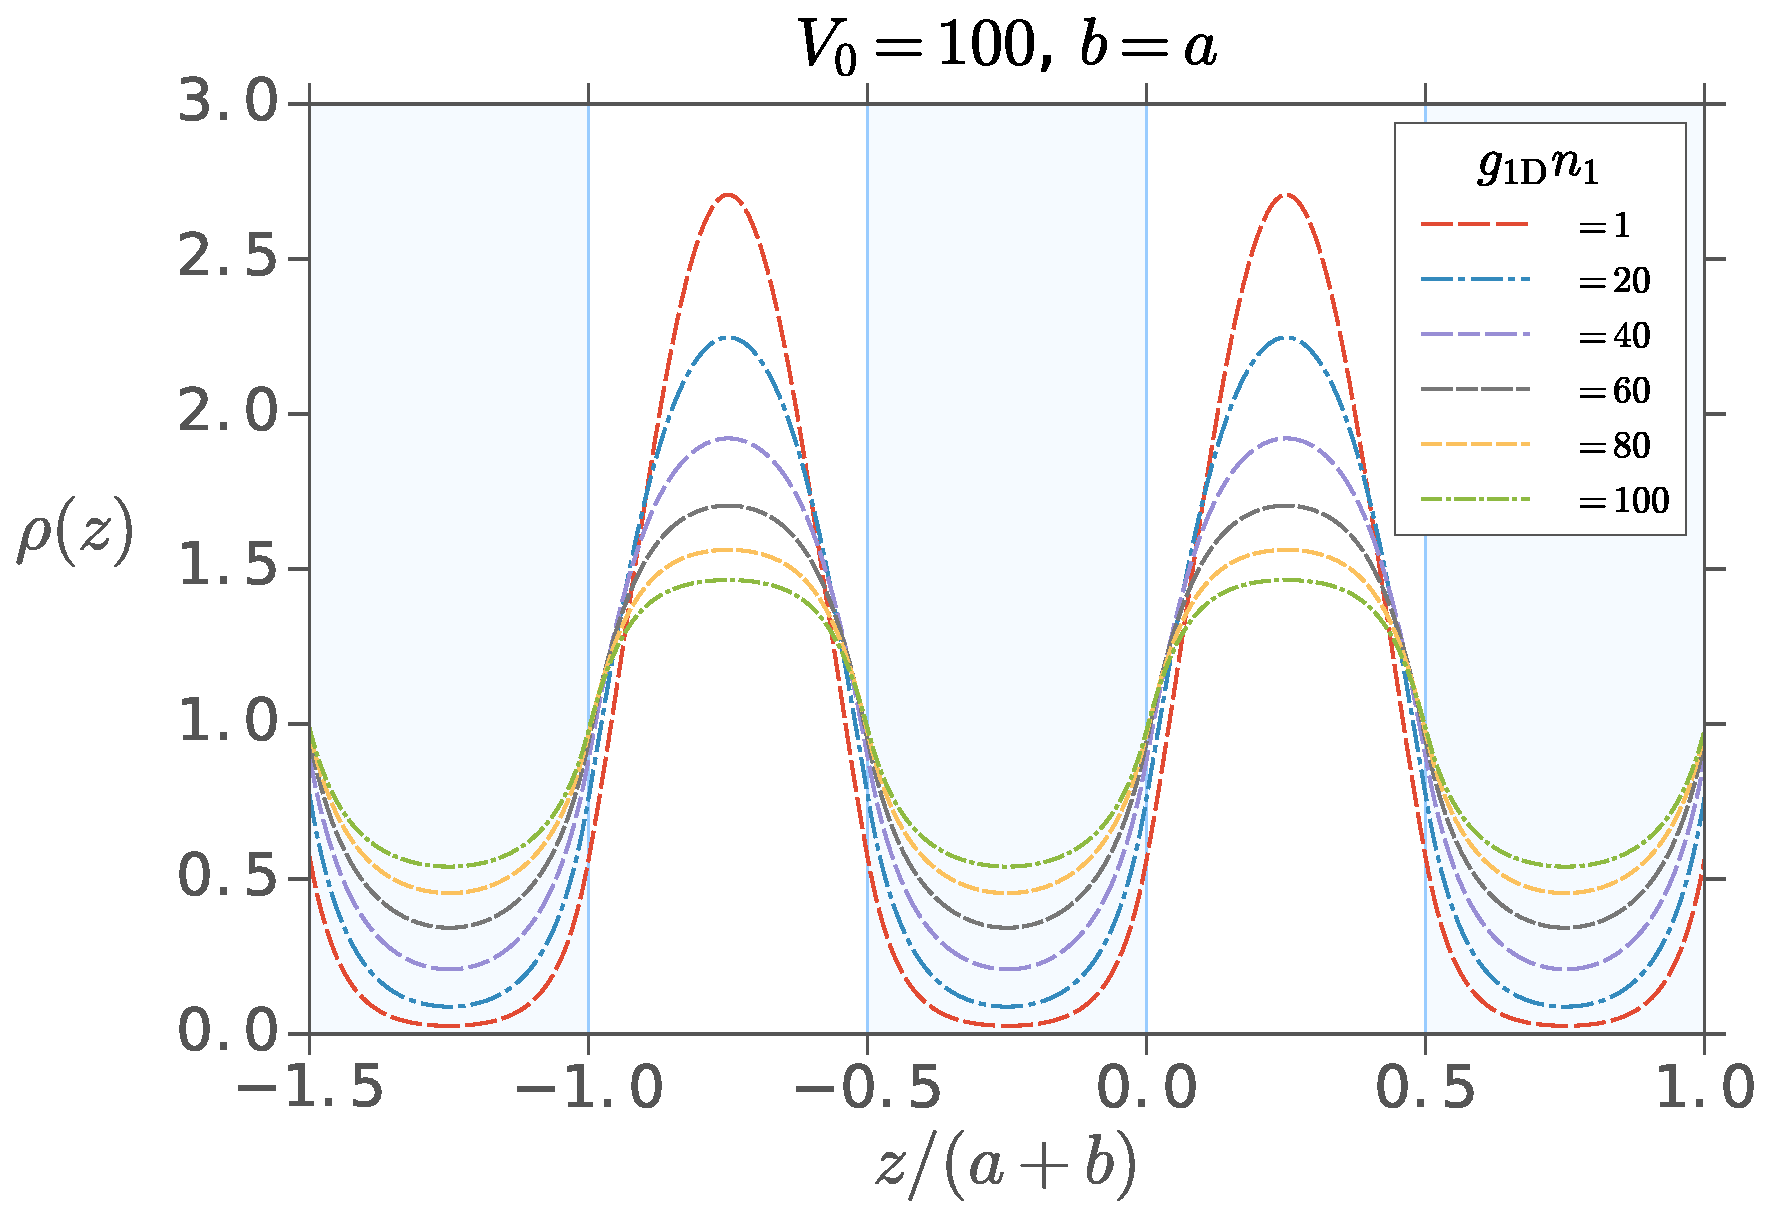
\includegraphics[width=0.75\linewidth]{./figures/density_profile_gp_u0-100_r-1}
  \caption{Density profile (normalized) for an interactive (repulsive) Bose gas
    within a multi-rods structure as a function of the position, for several
    values of the interaction parameter. Both the potential magnitude and the
    interaction parameter are given in units of $\hbar^2 / 2 m (a+b)^2$. The
    darker regions indicate the localization of the external potential
    barriers.}
  \label{fig:density-profile-gp-u0-100-r-1}
\end{figure}
%
The solution of the nonlinear system of equations
\eqref{eq:gross-pitaevskii-density-continuity},
\eqref{eq:gross-pitaevskii-density-derivative-continuity},
\eqref{eq:gross-pitaevskii-density-derivative-periodicity},
\eqref{eq:gross-pitaevskii-system-momentum},
\eqref{eq:gross-pitaevskii-chemical-equlibrium} and
\eqref{eq:gross-pitaevskii-normalization-condition} allow us to obtain the
density profile and the energy per boson of the diluted Bose gas.

The density profile when the potential magnitude is $V_0 = 100$ (in units of
$\hbar^2 / 2m(a+b)^2$) and $b/a = 1$ (barrier width equal to separation) as a
function of the position is shown in the figure
\ref{fig:density-profile-gp-u0-100-r-1}. In the picture appear several curves
each one for a different value of $\gonedim n_1$ which measures the magnitude of
the interaction between bosons: greater values mean stronger interactions. As
expected, the density is greater in the region between the barriers, and is
lower in the space where the external potential acts. Interestingly, as the
interaction increases the density differs greatly from the ideal case, and
becomes more and more uniform.

As a comparison, we found stationary solutions when the interaction parameter is
negative, as shown in the figure \ref{fig:density-profile-gp-u0-100-r-1-attr}.
The potential shape is the same as the plotted in
\ref{fig:density-profile-gp-u0-100-r-1}, but in this case the interaction
magnitude is negative and its absolute value increases progressively. In this
case there is a sharp localization of the particles in the midpoint between the
barriers, and a very strong depletion of the density in the region where the
potential is nonzero.
%
\begin{figure}[h!]
  \centering
  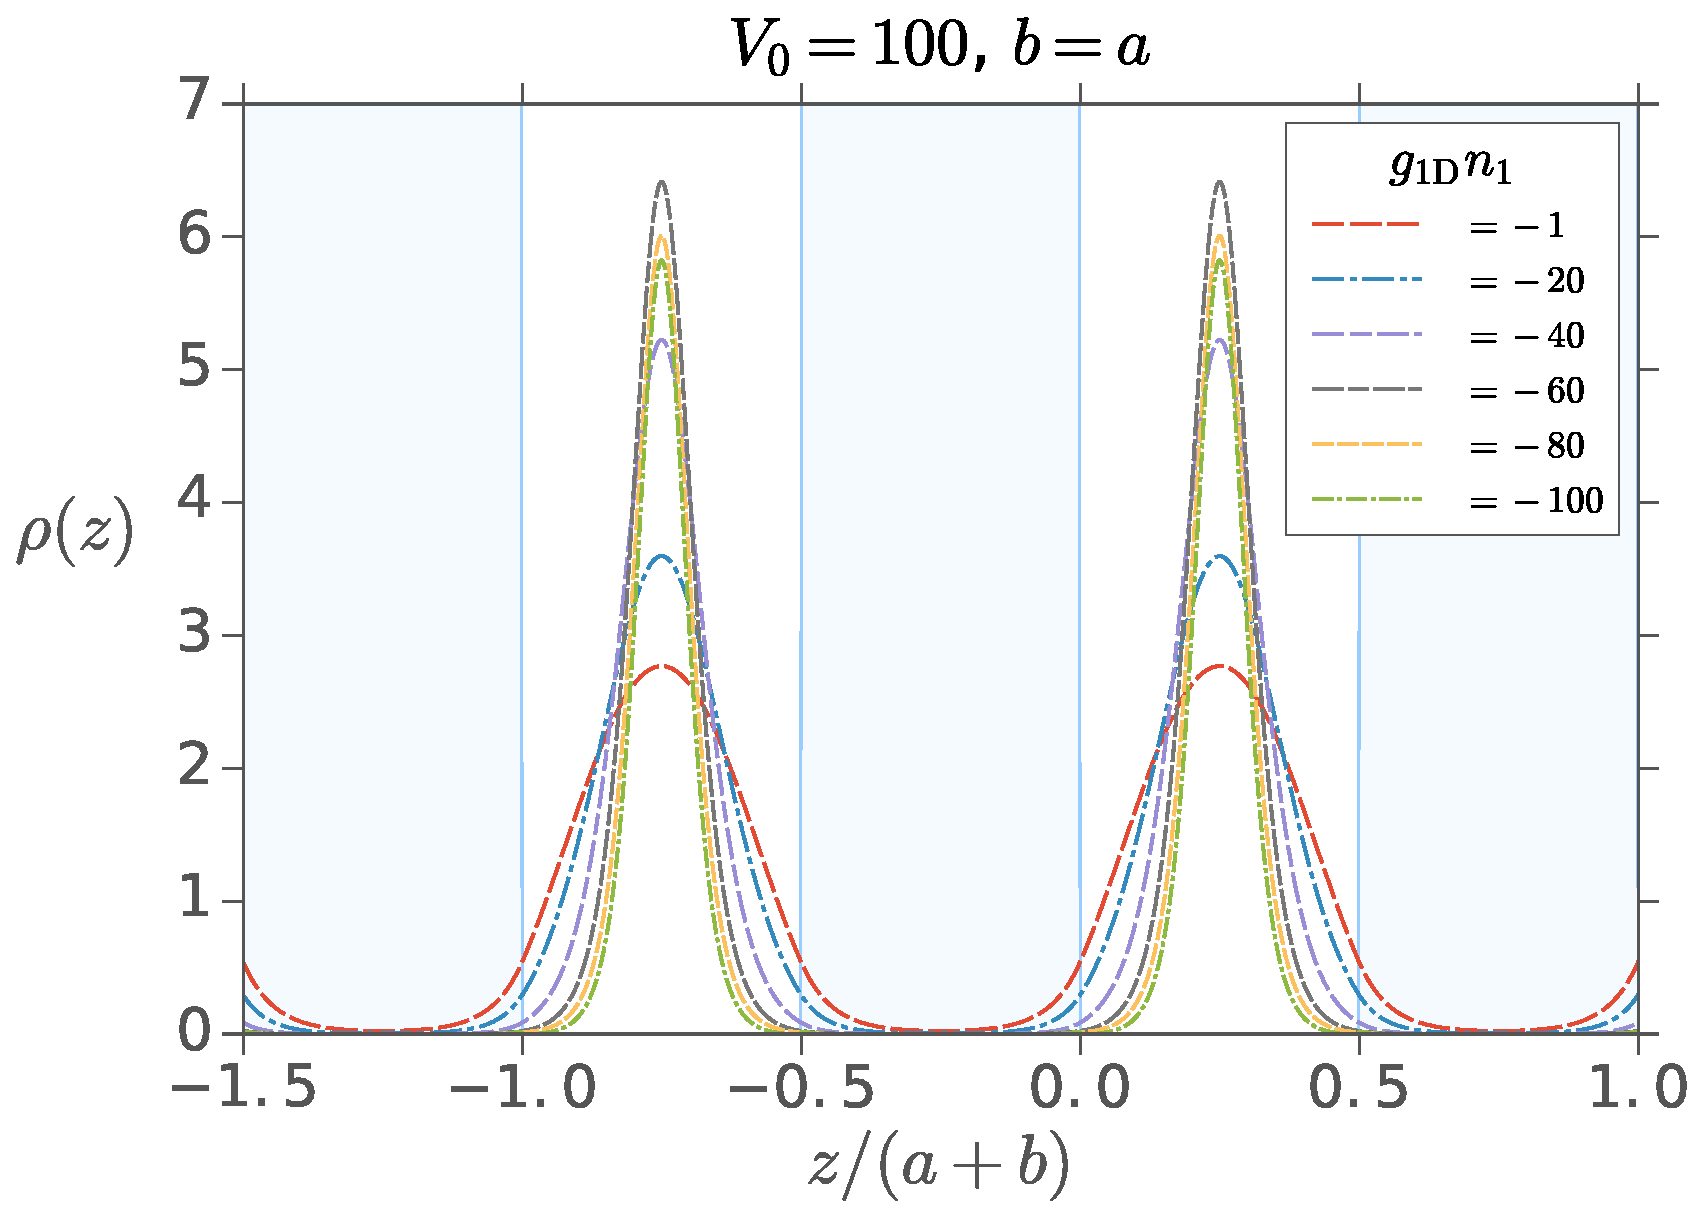
\includegraphics[width=0.75\linewidth]{./figures/density_profile_gp_u0-100_r-1_attr}
  \caption{Density profile (normalized) for an interactive (attractive) Bose gas
    within a multi-rods structure as a function of the position, for several
    values of the interaction parameter. Both the potential magnitude and the
    interaction parameter are given in units of $\hbar^2 / 2 m (a+b)^2$. The
    darker regions indicate the localization of the external potential.}
  \label{fig:density-profile-gp-u0-100-r-1-attr}
\end{figure}
%

The data obtained for the energy as a function of the interaction parameter
$\gamma = 2 / \densityone \asonedim$. There is a relation between the
Lieb-Liniger model parameter $\gamma$ and $\gonedim \densityone$, but in view of
the Eq. \eqref{eq:lieb-liniger-energy} it is necessary to fix the density of the
system in order to obtain the energy per boson of the gas. Furthermore, as we
are comparing the results obtained from mean-field theory with those predicted
by the Lieb-Liniger theory, we have to restrict ourselves to a very small
interval of values for $\gamma$. In figure
\ref{fig:gross-pitaevskii-energy-as-gamma-nb-40} we can see how the energy
predicted by the Gross-Pitaevskii equation solutions compares to the predictions
of the Lieb-Liniger theory, and how it changes as the external potential
magnitude increases.
%
\begin{figure}[t!]
  \centering
  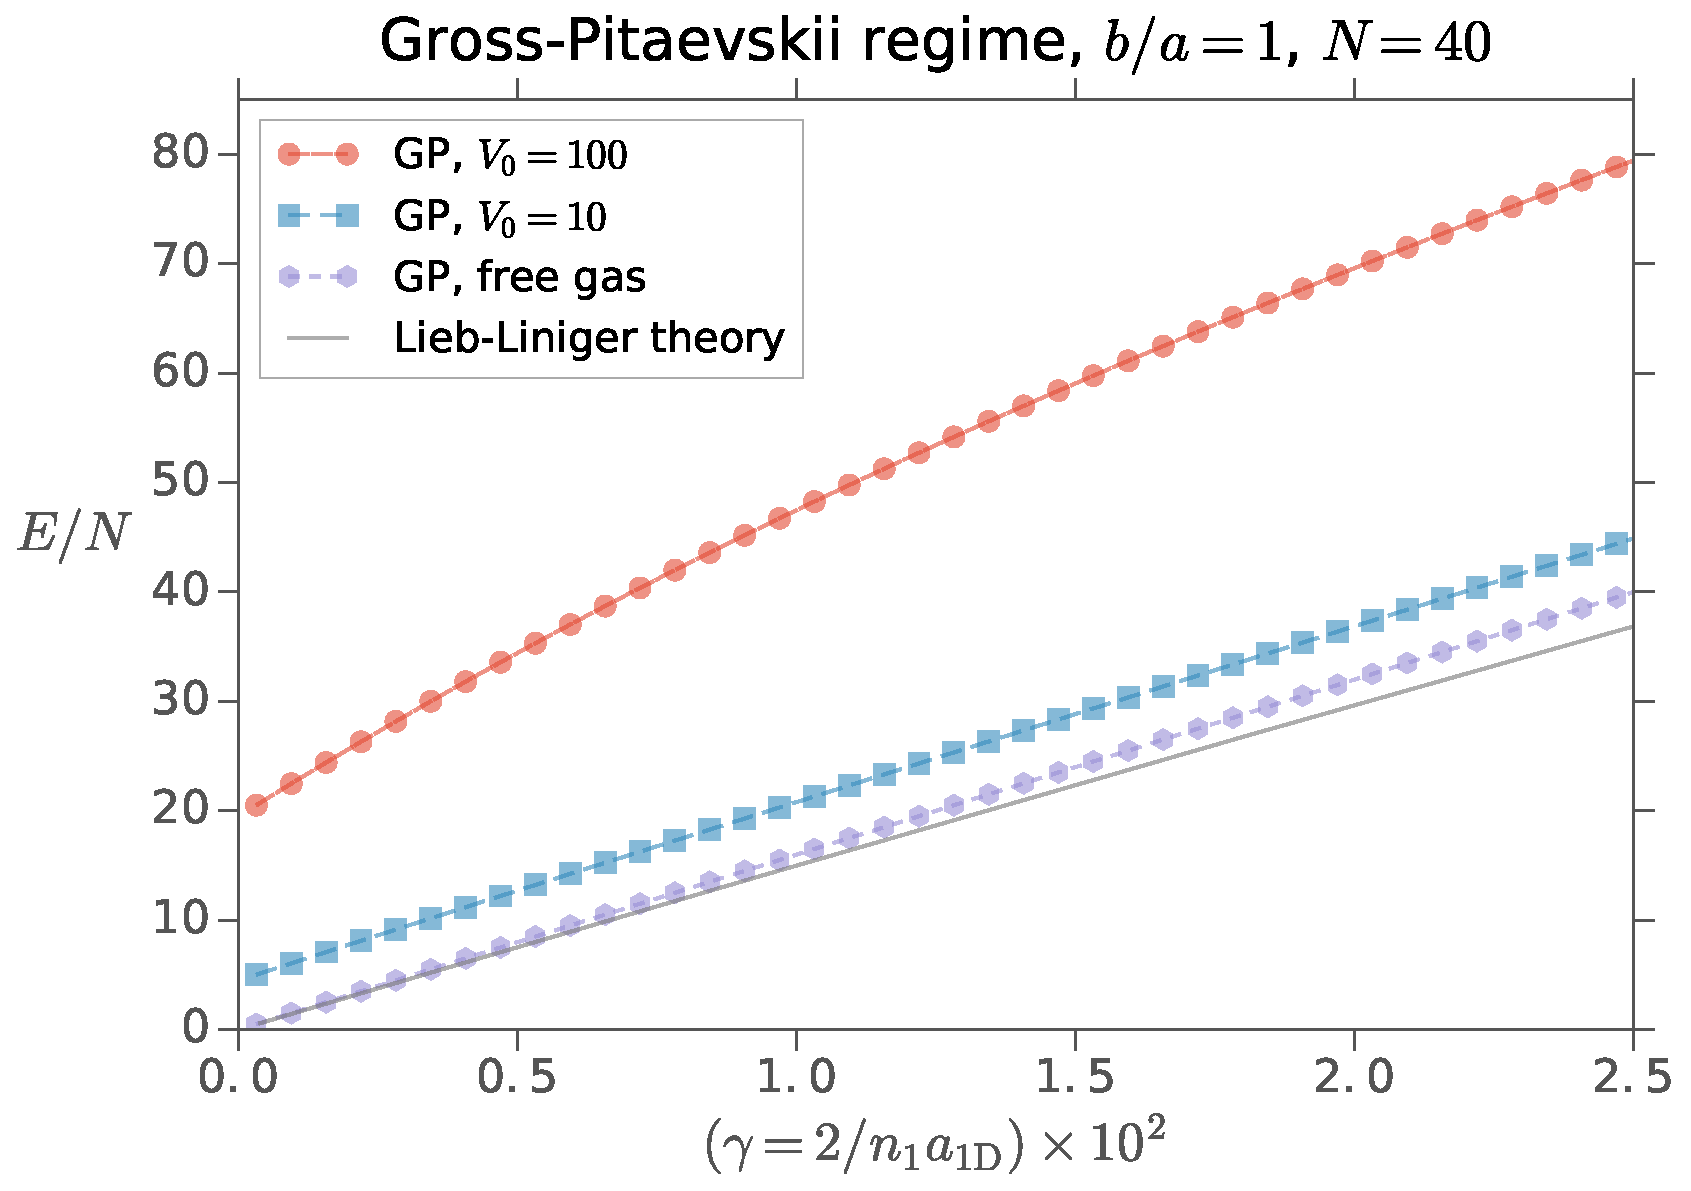
\includegraphics[width=0.75\linewidth]{./figures/gp_energy-as-gamma_Nb-40}
  \caption{Energy per boson (in units of $\hbar^2 / 2m(a+b)^2$) as a function of
    the Lieb gamma parameter obtained from the solution of the Gross-Pitaevskii
    equation in 1D \eqref{eq:gross-pitaevskii-energy-multirods} for different
    magnitudes of the external potential. The energy given by the Lieb-Liniger
    theory (no external potential) is shown as a solid line as a reference. The
    energy for zero external potential is plotted with hexagonal markers.}
  \label{fig:gross-pitaevskii-energy-as-gamma-nb-40}
\end{figure}
%
The mean-field theory applied to the particular case when the Kronig-Penney
potential magnitude is zero yields the expected result: $E / N = \gonedim
  \densityone / 2$. However even for the small values of $\gamma$ we have used,
its results differ from the Lieb-Liniger theory, and that difference becomes
larger as $\gamma$ does. It is clear that the applicability of the mean-field
regime is constrained to very small values of $\gamma$, or equivalently, to
enough large values of $\densityone \asonedim$.


